% ************************************************
\chapter{Graph Theory}\label{ch:Graph_theory} 
% ************************************************

A review of graph theory lays the foundation for the mathematical
considerations in this work. 

 In this chapter we review basic graph
theory and explain how these terms are applicable in the context of
biological neural networks. We begin with the definition of directed
graphs: %?? needs rework








% ######################################################################### %
% ------------------------------------------------------------------------- %
%                             Directed Graphs 
% ------------------------------------------------------------------------- %
% ######################################################################### %


\section{Directed graphs}\label{sec:directed_graphs}


%  \begin{definition}[Graph, Order] A \textbf{graph} is a pair of sets $G
% =(V,E)$, consisting of the \textbf{vertex set} $V(G)=V$ and the
% \textbf{edge set} $E(G)=E$, such that $E \subseteq V \times V$.  The
% number of vertices of a graph $G$ is its \textbf{order} $|G|$, the
% number of edges is denoted by $||G||$.  A graph of order $0$ or $1$ is
% called \textit{trivial}.
%   \end{definition}

%   The object of interest in my thesis will be directed pseudographs,
% but I will still have to think about how to
%   \begin{itemize}
%   \item call them, graphs, directed graphs, etc..
%   \item think about the weights(!!)
%   \item think about definitions
%   \end{itemize}


\begin{definition}[Directed graphs]
  \index{directed graph} \index{simple graph} \index{pseudograph}
  \index{multigraph} \index{loop graph}
  \label{def:directed_graphs}
  A \textit{directed pseudograph} $G$ consists of two finite
  %
  % Non-empty? -> No. Empty graph allowed for random 
  % graph process that adds edges and or vertices
  % 
  $V$, the \textit{set of vertices} of $G$, and $E$, the \textit{set
    of edges} of $G$, and two maps $ s,t: E \to V, $ the
  \textit{source} and \textit{target functions} of $G$. A
  \textit{directed multigraph} is a directed pseudograph without
  loops, that is the map $d = (s,t):E \to V^2$ already maps
  maps to $V^2\setminus\Delta_V$, where $V^2 = V \times V$ denotes the
  cartesian product and $\Delta_V = \{(x,x) \mid x \in V\} \subseteq
  V^2$ the diagonal. Similarily, a \textit{directed loop graph} is a
  directed pseudograph where $d$ is injective. Finally, a
  \textit{simple directed graph} can be defined as a directed
  pseudograph where $d$ is both injective and already maps to
  $V^2\setminus\Delta_V$.
\end{definition}

Thus, in simple directed graphs, neither parallel edges nor loops -
edges between the same vertex - are allowed, whereas directed
multigraphs and directed loop graphs admit one of them respectively.

\red{Say something about what "directed graph" means here, do all
  definition until random graphs work for all types of directed graphs?}

\begin{figure}[!htbp]
  \centering 
  \makebox[0.6\textwidth]{%
    \begin{overpic}[width=0.25\textwidth]{%
        tikz/directed_pseudograph.pdf}
      \put(-15,35){\small\textbf{A}}
    \end{overpic}
    \hfill
    \begin{overpic}[width=0.25\textwidth]{%
        tikz/directed_multigraph.pdf}
      \put(3,35){\small\textbf{B}}
    \end{overpic}
    }%
  \vfill
  \vspace{0.25cm}
  \makebox[0.6\textwidth]{%
    \begin{overpic}[width=0.25\textwidth]{%
        tikz/directed_loopgraph.pdf}
      \put(-15,35){\small\textbf{C}}
    \end{overpic}
    \hfill
    \begin{overpic}[width=0.25\textwidth]{%
        tikz/directed_simple_graph.pdf}
      \put(3,35){\small\textbf{D}}
    \end{overpic}
    }%
    \caption{%
      \textbf{Typical examples of the directed graph types}
      \textbf{A)} directed pseudograph \textbf{B)} directed
      multigraph \textbf{C)} directed loop graph \textbf{D)} simple
      directed graph.} %??
  \label{fig:directed_graph_types}
\end{figure}

Given a directed graph $G$, we denote with $V(G)$ the set of vertices
of $G$ and call it the \textbf{vertex set} of $G$. Analogously, the
\textbf{edge set} $E(G)$ of $G$ denotes the set of edges of $G$. This
means, for a directed graph specified as $G = (V,E,s,t)$, we
have $V(G) = V$ and $E(G) = E$.

A \textbf{morphism} $\phi: G \to H$, between two directed graphs
$G=(V_G,E_G,s_G,t_G)$ and $H=(V_H,E_H,s_H,t_H)$, consists of a pair of
maps $\phi_V: V_G \to V_H$ and $\phi_E: E_G \to E_H$, such that
\[
s_H \circ \phi_E = \phi_V \circ s_G \mathrm{\quad and \quad} t_H \circ
\phi_E = \phi_V \circ t_G,
\]
that is such that the following diagram commutes:
%
\begin{align*} 
  \xymatrix@+=1.3cm{E_G \ar^{t_G}@<0.66ex>[d] \ar_{s_G}@<-0.66ex>[d]
    \ar^{\phi_E}[r] & E_H \ar^{t_H}@<0.66ex>[d]
    \ar_{s_H}@<-0.66ex>[d]\\ V_G \ar^{\phi_V}[r] & V_H}
\end{align*}
%
A morphism $\varphi: G \to H$, between two directed pseudographs $G$
and $H$ is an \textbf{isomorphism}, if the maps $\varphi_V: V_G \to
V_H$ and $\varphi_E: E_G \to E_H$ are bijective. Two directed
pseudographs are called \textit{isomorphic} if there exists an
isomorphism inbetween them.

\begin{remark}
  The last definition implies that, if there exists an isomorphism
  $\varphi: G \to H$, an isomorphism $\psi: H \to G$ can be
  found. This isomorphism is, of course, easily constructed via
  $\psi_V: V_H \to V_G, v \mapsto \varphi_V^{-1}(v)$, $\psi_E: E_H \to
  E_G, e \mapsto \varphi_E^{-1}(e)$.
\end{remark}

\begin{definition}[Weighted directed graphs]
  \index{weighted graph}
  An \textit{edge-weighted directed graph} is a directed graph $G$ along
  with a mapping $\omega: E(G) \to \mathbb{R}$, called the
  \textit{weight function}. Similarly, a \textit{vertex-weighted
    directed graph} is a directed graph with a mapping $\nu: V(G) \to
  \mathbb{R}$.
\end{definition}

\begin{remark} \red{(heavy draft)}

  % 
  % Think about
  %  - synaptic integration (non-linear)
  %  - self excitation, interessed in axonal-dendritic connections, so
  %    probably not for structure but maybe dynamics?
  % 

  % Title: A directed graph category for biological neural networks

  Certainly, a weighted directed pseudograph is the most fitting
  mathematical modelling to the biological situation, since self
  connections and multiple synapse are not only plausibel (source?)
  but the rule. However there is one abstraction we can make by adding
  together the synaptic weights - NEST is doing it. While linear
  synaptic integration was shown to be, it is a prevalent model in
  network (ref Nest).\\ 

  Also think about \textbf{inhibitory, excitatory}. Suggestion: edge
  weights $\omega: E(G) \to \mathbb{R}^{+}$ \textbf{and} vertex
  weights $\nu: V(G) \to \{-1, 1\}$. Synaptic weight $\mathrm{syn}(e)$
  for edge $e$ is then \[\mathrm{syn}(e) = \nu(s(e))\,\omega(e).\]
  Benefit: Synapse from one neuron are either excitatory or inhibitory
  but not mixed as in bio.
\end{remark}


\begin{remark}[Equivalent definiton for directed loop graphs]

  A directed loop graph $G$ can be equivalently defined as a pair of
  finite\red{(, non-empty?)} sets $V$, the \textit{set of vertices} of
  $G$, and $E \subseteq V^2$ the \textit{set of edges} of $G$. For an
  edge $(x,y) \in E$, we call $x$ the \textit{source} and $y$ the
  target of the edge $(x,y)$.

  Source and target functions are then uniquely determined as the
  projections on the first and second component, $s = \mathrm{pr}_1, t
  = \mathrm{pr}_2: E(G) \to V.$ Conversely, the edge set $E(G)
  \subseteq V^2$ can be determined from the source and target
  functions as $E:=\{(s(e),t(e)) \mid e \in E\}$. The trivial identities
  $(x,y) = (\mathrm{pr}_1(x,y),\mathrm{pr}_2(x,y))$ and
  $\mathrm{pr_1}(s(e), t(e)) = s(e)$ with $\mathrm{pr_2}(s(e), t(e)) =
  t(e)$ quickly verify the equivalence of the definitions.

  Given a directed loop graph $G$, we often assume the graph to be
  given in this form and write edges as $e=(x,y)$. Note that this
  concept is more complicated to introduce for directed pseudographs,
  since parallel edges $e$ and $e'$ should to be differentiated in the
  egde set of $G$, establishing the need for $E(G)$ to be a multi- or
  indexed set, notions we are trying to avoid in this document.

\end{remark}



% A given directed loop graph $G = (V,E,s,t)$, can always be
% represented by a canonical isomorphic directed loop graph $G' =
% (V,E')$, where $E':=\{(s(e),t(e)) | e \in E\} \subseteq V^2$. For a
% directed loop graph $G'$ in canonical form, the source and target
% functions $s',t'$ do not need to be specified, since they are uniquely
% determined as the projections on the first and second component, $s' =
% \mathrm{pr}_1, t' = \mathrm{pr}_2$. Wait, not so easy because
% multi-sets, however add synaptic strength of parallel edges to make
% directed loop-graphs! (Bang-Jensen)



From now on any \textit{directed graph} is assumed to be a directed
loop graph. Although most, if not all, concepts work for directed
pseudographs just as well, we want to start to heavily use the
canonical edge representation, which when talking about pseudograps
makes problems as mentioned before.

\begin{remark}[More Notation] 
  \red{- Check, do I really need this?} For a pair of vertex sets $X,Y
  \subseteq V(G)$ of a directed graph $G$ we write
  \[
  (X,Y)_G = \{(x,y) \in E(G) | x \in X, y \in Y \}
  \]
  for the set of edges with source in $X$ and target in $Y$. For
  vertex sets with a single element $X = {x}$, we also write $(x,Y)_G$
  and mean the edges with source $x$ and target in $Y$.
\end{remark}


\begin{definition}[In- and out-degree]  
  \index{in-degree}\index{out-degree}
  For a directed graph $G$ the \textbf{in-degree} $d^-_G(x)$ of a
  vertex $x$ is defined as the number of edges of $G$ with target $x$,
  that is
  \[
  d^-_G(x) = \left|(V(G),x)_G\right|.
  \]
  Similarily, the \textbf{out-degree} $d^+_G(x)$ of $x$ is defined as
  \[
  d^+_G(x) = \left|(x, V(G))_G\right|,
  \]
  the number of edges in $G$ with source $x$.
\end{definition}

\begin{remark}[Side]
  In some literature about directed graphs (Bang-Jensen), loops are
  \textit{not} counting towards the in- or out-degree of vertex. In
  the light of neural network however, we specifically want to count
  loops as well.
\end{remark}

A basic property of the in- and out-degree in directed graphs is that
number of in-degrees of every vertex, as well the sum of every
out-degree, equal the total number of edges:

\begin{proposition}
  In every directed graph $G$, we have
  \[
  \sum_{x \in V(G)} d^-(x) = \sum_{x \in V(G)} d^+(x) = | E(G) |.
  \]
\end{proposition}

\begin{proof}
  Since $(V(G),x)_G \cap (V(G),y)_G = \emptyset$ for $x \ne y$, we can
  write
  \[
  \sum_{x \in V(G)} d^-(x) = \left| \bigcup_{x \in V(G)} (V(G),x)_G
  \right| = \left| (V(G),V(G))_G \right| = | E(G) |.
  \]
  Analogously for the out-degree.
\end{proof}








% ######################################################################### %
% ------------------------------------------------------------------------- %
%                          Walks and Distances
% ------------------------------------------------------------------------- %
% ######################################################################### %


\section{Walks and distances}\label{sec:walks_and_distances}


Let $G$ be a directed graph \red{(what does it mean here?)}. A
\textbf{walk} $W$ in $G$ is an alternating sequence
$(x_1,e_1,x_2,e_2,x_3,\ldots,x_{n-1},e_{n-1},x_n)$ of of vertices
$x_i$ and edges $e_i$ from $G$, such that
\[
s(e_i) = x_i \quad \mathrm{and} \quad t(e_i) = x_{i+1}, \:\,
\mathrm{for}\, i=1,..,n-1,
\]
that is, such that the vertices are connected by the edges inbetween
them. We denote the set of vertices $(x_1,\ldots,x_n)$ of $W$ as
$V(W)$ and the sequence of edges $(e_1,\dots,e_{n-1})$ as $E(W)$
\red{(need it?)}.

The vertices $x_1$ and $x_n$ are called the \textit{end vertices} of
$W$ and we also say that $W$ is an $(x,y)$-walk. The \textbf{length}
of $W$ is defined as the length of the sequence of edges; a walk
consisting of only one vertex has length zero. \red{ colon, really?}


\begin{definition}[Distance]
  The \textbf{distance} of two vertices $x$,$y$ in a directed graph
  $G$ \red{(means?)}, is defined as the minimum length of an
  $(x,y)$-walk, if any such walk exists, otherwise
  $\operatorname{dist}(x,y)=\infty$. In short,
  \[
  \operatorname{dist}(x,y) = \inf \{|E(W)| \mid
  W\,\mathrm{is}\,(x,y)\mathrm{-walk}\}.
  \]
  \red{$|E(W)|$ is not explained. Necessary?}
\end{definition}

\begin{proposition}
  The distance function $\operatorname{dist}: V(G) \times V(G) \to
  \mathbb{N}$ of a directed graph $G$ satisfies the triangle equality,
  \[
  \operatorname{dist}(x,z) \le \operatorname{dist}(x,y) +
  \operatorname{dist}(y,z), \:\: \mathrm{for}\:\, x,y,z \in V(G).
  \]
\end{proposition}

\begin{proof}
  Let $x,y,z$ be vertices in $G$. If either no $(x,y)$-walk or
  $(y,z)$-walk exists, the inequality holds by definition. Other wise,
  let $W$ be an $(x,y)$-walk of minimal length and let $U$ be a
  $(y,z)$-walk of minimal length. Certainly, by concatenating $W$ and
  $U$ we obtain an $(x,z)$-walk of length $|E(W)| + |E(U)| =
  \operatorname{dist}(x,y) + \operatorname{dist}(y,z)$, proofing
  that \[ \operatorname{dist}(x,z) \le \operatorname{dist}(x,y) +
  \operatorname{dist}(y,z).
  \]
\end{proof}





%   \begin{definition}[Neighbour, adjacent] Two \textbf{vertices} $x,y \in
% V(G)$ of $G$ are called \textit{adjacent} or \textit{neighbours} if
% there is an edge between $x$ and $y$, $(x,y) \in E(G)$. Two
% \textbf{edges} $e \neq f$ are \textit{adjacent} if they have an end in
% common.
%   \end{definition}


More to do:

\begin{itemize}
\item summarize category of directed (weighted) pseudographs
\item weights!
\item vertices will also be called nodes and neurons, edges will also
  be connections or synapses.
\item subgraphs
\item \sout{vertex set, edge set $E(G), V(G)$.}
\item $\omega(e)$ is weight, connection strength or synaptic weight
  (as a side remark
\item extend to category of weighted directed pseudographs
  (isomorphisms)
\item path
\item adjacency matrix
\item converses of graph related to opposite category?
\item \sout{in- and out-degree}
\item \sout{triangle inequality for distance, $\mathrm{dist}(x,z) \leq
  \mathrm{dist}(x,y) + \mathrm{dist}(y,z)$}
\end{itemize}



References for this chapter:
\url{http://nlab.mathforge.org/nlab/show/graph},
\url{http://nlab.mathforge.org/nlab/show/quiver}, \parencite{Bang-Jensen_Digraphs}








% ######################################################################### %
% ------------------------------------------------------------------------- %
%                          Random Graph Theory
% ------------------------------------------------------------------------- %
% ######################################################################### %


\section{Random Graph Theory}\label{sec:random_graph_theory}


From this chapter on, as it is common and practical when talking about
random graph models, we move away from the abstract notion
%------------------------------------------------
\marginpar{focus on labeled, simple directed graphs}
%------------------------------------------------ 
of graphs and their equivalence classes and consider \textit{labeled
  graphs}, where the edge set of a graph with $n$ vertices takes the
form $V = \{1,\ldots,n\}$. Simple directed graphs constitute the
fundamental mathematical object underlying the concepts developed in
this work and if not specified otherwise, all graphs are assumed to be
labeled and simple directed.
%?? Focus on simple directed graphs!

The concept of a random graph was first formally introduced by
\textcite{Erdos1959}. In their $G(n,N)$ model, a graph with $n$
vertices and $N$ edges is randomly and with equal probability selected
from the set of such possible graphs. In the same year
\textcite{Gilbert1959} independently introduced his $G(n,p)$ model,
realizing edges between vertex pairs with a fixed probability $p$. The
two models are closely related \parencite{Luczak1990} and overlap in
literature, both at times being to referred to as
\textit{Erd\H{o}s-R\'{e}nyi graphs}. Here we focus on the $G(n,p)$
model, as it closer in concept to a computational implementation of a
random graph. Defining it in detail in \ref{def:gilbert_random_graph},
we will refer to the random graph model as the \textit{Gilbert random
  graph model}.

\index{random graph}%
In general, a random graph model is a probability space over a set of
graphs \parencite{Janson_Random-graphs}. Rather than specifying the
sample space and probability
%------------------------------------------------
%\marginpar{definition as probability space or random process}
%------------------------------------------------ 
measure explicitly, random graph models are often defined by a random
process that generates such graphs, leaving probability measure and
sample space implicit \parencite{Bollobas_Random-graphs}. The term
\textit{random graph}, in the graph theoretical context, refers to the
random graph model itself. Especially in the computational context
however, a random graph often refers to a single graph generated by a
random process. Here we try to avoid this ambiguity and strictly refer
to the mathematical object as a random graph model.

Keeping in mind that the term \textit{graph} now refers to labeled,
simple directed graphs if not otherwise specified we define $G^n$ to
be the set of simple directed graphs with $n$ vertices,
\[
G^n := \{G \mid G\,\mathrm{\,graph},\, |V(G)| = n\}.
\]
We first introduce Gilbert's random graph model $G(n,p)$ by explicitly
defining a probability space over $G^n$ and show later how the model
may be realized as a random process. 

\begin{definition}[Gilbert random graph model]
  \label{def:gilbert_random_graph} \index{Gilbert random graph model}
  Let $n\in\mathbb{N}$ and $0\leq p \leq 1$. The \textit{Gilbert
    random graph model} $G(n,p)$ is a discrete probability space over
  $G^n$ with event space $\mathcal{P}(G^n)$ and probability measure
  $P$, such that every graph $G$ with $\abs{E(G)}=k$ edges appears
  with equal probability%
  \[%
    P(G) = {p^k(1-p)^{n(n-1)-k}},%
  \]%
  for $0 \leq k \leq n(n-1)$. 
\end{definition}

\begin{remark}Clearly $G(n,p)$ is well-defined, as there exist $\binom{n(n-1)}{k}$
distinct labeled graphs with $n$ vertices and $k$ edges and thus 
\[
  \sum_{G \in G^n} P(G) =  \sum_{k=0}^{n(n-1)}  \binom{n(n-1)}{k}
  p^k(1-p)^{n(n-1)-k} = 1, % = (p+(1-p))^{n(n-1)}
\]
after the binomial theorem.
% Which sigma algebra -> power set (discrete probability space)
\end{remark}


Equivalently, the Gilbert random graph model can be defined as a
stochastic process;
%------------------------------------------------
\marginpar{equivalent definition as random process} 
%------------------------------------------------ 
to an empty graph with $n$ vertices, for each of the $n(n-1)$ vertex
pairs an edge is added at random and independently with probability
$p$. The probability to obtain a specific graph $G$ with $k$ edges is
then obviously $p^k(1-p)^{n(n-1)-k}$, already proofing the
equivalence, since assuming a process as above with edge probability
$p'$ such that the induced probability measure on $G^n$ equals
$P$ from \ref{def:gilbert_random_graph}, already yields $p = p'$ in
the choice of $n=2$ and $k=1$. 

\begin{proposition}
  In- and out-degree distribution of vertices in the Gilbert random
  graph model are binomial.
\end{proposition}
%
\begin{proof}
  Let $X$ be a random variable on the random graph model, mapping to
  the in-degree (out-degree) $d_G(v)$ of a vertex $v$ of a graph $G
  \in G^n$. There are $n-1$ other vertices that, with probability $p$,
  project to $v$ (receive input from $v$), thus
  \[
    P(X=k) = \binom{n-1}{k} p^k (1-p)^{n-1-k},%
  \]%
  % $X: G^n \to \mathbb{R}, G \to |E(G)|$, discrete random variable,
  % with probability distribution $\operatorname{B}_{n(n-1),p}$.
  % \[
  % \operatorname{B}_{n(n-1),p}(k) = \binom{n(n-1)}{k} p^k(1-p)^{n(n-1)-k}
  % \]
  showing that $P^X = \mathcal{B}_{n-1,p}$.
\end{proof}

The Gilbert random graph model is therefore also often referred to as
\textit{binomial random graph}\index{binomial random
  graph}. %\parencite{Janson_Random-graphs}
As typical neuronal networks are large ($n \geq 10^3$) with sparse
connectivity ($p \approx 0.1$), in- and out-degree distribution can be
approximated by a Poisson distribution, $P^X(k) \approx
\operatorname{Pois}_{\lambda}(k)$, with $\lambda = (n-1)p$, after the
Poisson limit theorem.

Most results in the study of random graph models consider $n\to
\infty$. In this study we are mostly interested in patterns of
connectivity that arise in local circuits, leaving behind limit
considerations and employ the Gilbert random graph model as a
reference for the development of more detailed and specific random
graph models.








% ######################################################################### %
% ------------------------------------------------------------------------- %
%                            Geometric Graphs
% ------------------------------------------------------------------------- %
% ######################################################################### %


\section{Geometric Graphs}\label{sec:geometric_graphs} 


The theory of geometric graphs address the embedding of graphs in
$\mathbb{R}^d$.  Planar graphs are graphs that can be drawn on a
surface with their edges drawn as straight lines between the vertices,
such that no two lines intersect
\parencite{Diestel_Graph-theory}. %Maybe West?
Here we are interested in graphs embedded on surface. In the models
introduced, connectivity then depends on geometric properties, such as
distance between nodes or relative orientation between vertices. The
basic graph type to allow for such connectivity rules is a geometric
graph.

\begin{definition}[Geometric directed graph]
  \index{geometric graph} 
  A \textit{geometric directed graph}
  $G_{\Phi}$ is a directed graph $G$ paired with a map
  \[
    \Phi:V(G) \to [0,1]^2,
  \]
  representing vertex positions on the unit square.
\end{definition}

This definition diverges from the usual notion of a geometric graph,
which determines the existence of edges only between nodes within a
spatial distance $x$ in a specified
norm \parencite{Penrose_Geometric-graph}. Moreover, geometric graphs
are usually only discussed in the context of random graph models, a
concept first introduced by \textcite{Gilbert1961}. Denote the set of
geometric graphs with $n$ edges by $G_{\Phi}^n$. The spatial embedding
of geometric graphs allows us to define (random) connectivity
depending on vertex positions and inter-vertex distances.  Central to
this study is the distance-dependent random graph model, in which
edges are added with probability $p(x)$ depending on the distance $x$
between vertex pairs:

\begin{definition}[Distance-dependent random graph model]
  \index{distance-dependent!random graph model}
  Let $n \in \mathbb{N}$ and $C: [0,\sqrt{2}] \to [0,1]$ a
  continuous %?? C0 analytic?
  map.  A \textit{distance-dependent geometric random graph model}
  $G_{\Phi}(n,C)$ is a random graph model over $G^n_{\Phi}$, generated
  by distributing uniformly at random the $n$ vertices on the unit
  square and adding an edge from $v$ to $w$ for each vertex pair $(v,w) \in
  {V(G_{\Phi})}^2 \setminus \Delta_{V(G_{\Phi})}$ with a
  probability $C(x)$, depending on the distance $x = \norm{\Phi(v) -
    \Phi(w)}$ between the vertices.
\end{definition}

We call the function $C$ the graph's \textit{distance-dependent connection
  probability profile}\index{distance-dependent!connection
  probability}.
%------------------------------------------------
% \marginpar{profile $C$ and distance distribution determine
%   connectivity}
%------------------------------------------------
 Clearly, connectivity statistics in the
distance-dependent graph model intrinsically depend on the choice
$C$. To develop a thorough understanding of connectivity in the
model however, mapping the distribution of inter-vertex distances is
equally important. Here we calculate the distribution of the distance
between two random points in a square of side-length~$s$. Being able
to identify distributions of transformed random variables is integral
to the calculation:

\begin{lemma} \label{lemma:transform_random_variable} 
  Let $X,Y$ be independent continuous random variables with values in
  $\mathbb{R}$, denote with $f_X$ and $f_Y$ their probability
  distribution functions.%
  \begin{enumerate}[label=(\arabic*),ref=(\arabic*), itemsep=-0.6cm]
    \item The distribution of the random variable $X+Y$ is given by
      the probability density function%
      \[%
        f_{X+Y}(x) = \int_{\mathbb{R}} f_X(z) f_Y(z-x)\, dz.  
      \]% 
    \item The distribution of the random variable $X^2$ is given by
      the probability density function
      \[
        f_{X^2}(x) = %
        \begin{cases} 
          \frac{1}{2\sqrt{x}}\left(f_X(\sqrt{x})+f_X(-\sqrt{x})\right)
           & x > 0 \\           0     & x \leq 0 \\
        \end{cases}
      \]
    \item Let $X$ only take positive values. Then the distribution of
      the random variable $\sqrt{X}$ is given by the probability
      density function
      \[
        f_{\sqrt{X}}(x) = %
        \begin{cases}
          2x f_X(x^2) & x \geq 0 \\0   & x < 0 \\
        \end{cases}
      \]
  \end{enumerate}
\end{lemma}
%
% \begin{proof}
% Hello Proof
% \end{proof}

\begin{theorem} \label{theorem:distance_square}
  Let $D$ be a random variable mapping to the distance of
  two random points in the square $[0,s]^2$ of side-length $s$. Then the
  distribution of $D$ is given by the probability density function
  \vspace{0.25cm}
  \begin{align}\label{eq:distance_square}
    f(x) = \begin{cases} \frac{2 x^4 - 8 s x^3 + 2 \pi s^2 x}{s^4} & x \in
      [0,s]\\ \frac{H(x)}{s^4} & x \in [s,s\sqrt{2}),\\0 & x \notin [0,s\sqrt{2})
               \end{cases}
  \end{align}
  where
  \[
    H(x)=8 s x \sqrt{x^2-s^2} - 2x^3  
          - 4 s^2 x \left(1+\arcsin\left(1-\frac{2 s^2}{x^2}\right)\right).
  \]
\end{theorem}
%
\begin{proof}
  We follow the approach described by \textcite{Moltchanov2012}.
  Consider two independently and uniformly distributed random points
  $p_1 = (x_1,y_1)$ and $p_2 = (x_2,y_2)$ in $[0,s]^2$. The distance
  between $p_1$ and $p_2$ is given as
  \[
    \norm{p_1 - p_2} = \sqrt{(x_1 - x_2)^2 + (y_1 - y_2)^2}.
  \]
  As a first step we calculate the distribution for $\Delta_x = x_1 -
  x_2$. 
  % ------------------------------------------------
  % \marginpar{distribution for $\Delta_x = x_1 -  x_2$} 
  % ------------------------------------------------
  Denote with $f_{\Delta_x}$ its probability density. Then, since
  $f_{-x_2}(z) = f_{x_2}(-z)$,
  \begin{align}\label{eq:f_delta_x}
    f_{\Delta_x}(d) = f_{x_1 + (-x_2)}(d) = \int_{\mathbb{R}}  f_{x_1}(z)
    f_{x_2}(z-d)\, dz
  \end{align}
  after Lemma~\ref{lemma:transform_random_variable}.  % Klenke 14.19
  Density functions for $x_1$ and $x_2$ are given by
  \[
    f_{x_1}(z) = f_{x_2}(z) = %
    \begin{cases} 
      \frac{1}{s} & \mathrm{for} \, z \in  [0,s] \\
      0           & \mathrm{otherwise}.
    \end{cases}
  \] 
  Thus we may only obtain non-zero values in (\ref{eq:f_delta_x}) for $d
  \in (-s,s]$, as otherwise either one of the factors in the integrand
  is zero. In full we obtain the triangular distribution \parencite{Simpson1755},
  \begin{align*}
    f_{\Delta_x}(d) =  \begin{cases}
                         0 & d \notin (-s,s] \\
                         \frac{s+d}{s^2} & d \in (-s,0] \\
                         \frac{s-d}{s^2} & d \in (0,s].\\
                       \end{cases}
  \end{align*}  
  %
  Next we calculate the distribution for $\Delta_x^2 =
  (x_1-x_2)^2$. Using Lemma~\ref{lemma:transform_random_variable} once
  again we obtain for $d>0$
  \begin{align*}
    f_{\Delta_x^2}(d) & = \frac{1}{2\sqrt{d}}
    \left(f_{\Delta_x}(\sqrt{d}) + f_{\Delta_x}(-\sqrt{d})\right) \\
    & = \frac{1}{2\sqrt{d}} \left(\frac{s-\sqrt{d}}{s^2} +
      \frac{s+\left(-\sqrt{d}\right)}{s^2}\right) = \frac{1}{s\sqrt{d}} - \frac{1}{s^2},
  \end{align*}
  and $f_{\Delta_x^2}(d) = 0$ for $d \leq 0$. Note that of course,
  $f_{\Delta_x^2} = f_{\Delta_y^2}$ and we will refer to this density
  function as $f_\Delta^2$. Convolution yields again the probability
  density function for the sum of the random variables $\Delta_x^2$
  and $\Delta_y^2$,
  \begin{align*}%\label{eq:f_DeltaSum}
    f_{\Delta_x^2 + \Delta_y^2}(d) = \int_{\mathbb{R}} f_{\Delta^2}(z)
    f_{\Delta^2}(d-z)\, dz.
  \end{align*}

  Finally Lemma~\ref{lemma:transform_random_variable} lets us compute
  \begin{align*}%\label{eq:f_D}
  f_D(d) = f_{\sqrt{\Delta_x^2 + \Delta_y^2}}(d) = 2d\, f_{\Delta_x^2 +
    \Delta_y^2}(d^2),
  \end{align*}
  for $d \geq 0$, yielding expression (\ref{eq:distance_square}) for
   probability density function of $D$
   (Mathematica~\ref{mathematica:distances}, \ref{mathematica:comparison}). 
  % Otherwise, of course, $f_D(d) = 0$. Computing the
  % last two steps
  % % steps  (\ref{eq:f_DeltaSum}) and (\ref{eq:f_D}) 
  % in  Mathematica (see \autoref{mathematica:distances})
  % yields then expression (\ref{eq:distance_square}) for
  % probability density function of $D$. 
\end{proof}

The distribution for the distance between two random points in the
unit square $[0,1]^2$, is then obtained from
(\ref{eq:distance_square}) by setting $s=1$. The probability
density function $f$ becomes
  \begin{align}\label{eq:distance_unit_square}
    f(x) = %
      \begin{cases} 
        2 x^3 - 8 x^2 +  2 \pi x 
          & x \in [0,1) \vspace{0.15cm}\\ 
        8x \sqrt{x^2-1}-2x^3\\ 
        -4x- 4x\arcsin\left(1-\frac{2}{x^2}\right) 
          & x \in [1,\sqrt{2})
           \end{cases}
  \end{align}
  %
  % \begin{align}\label{eq:dist_pdf}
  %   f(x) = \begin{cases} 2 \pi x - 8 x^2 + 2 x^3 & x \in
  %     [0,s)\\ \begin{aligned} &8 x \sqrt{-1+x^2}-4 x-2 x^3\\ &-4 x
  %     \left(\frac{1}{\sqrt{-1+x^2}}\right)+4 x
  %     \arctan\left(\frac{1}{\sqrt{-1+x^2}}\right) \end{aligned}& x \in (1,\sqrt{2})
  %          \end{cases}
  % \end{align}
  % 
 
Plotting $f$ in combination with the results of a numerical simulation
($10000$ points randomly distributed on unit square, extracted
distances binned to a of width $\sqrt{2}/15$) verifies our calculation: 
%
%------------------------------------------------
\marginpar{\vspace{1.8cm}\\ label:
  \smtcite{01a179d9}\\ \smallskip More about labels
  in Appendix~\ref{sec:reproducibility}} 
%------------------------------------------------
\begin{figure}[H]
  \centering
  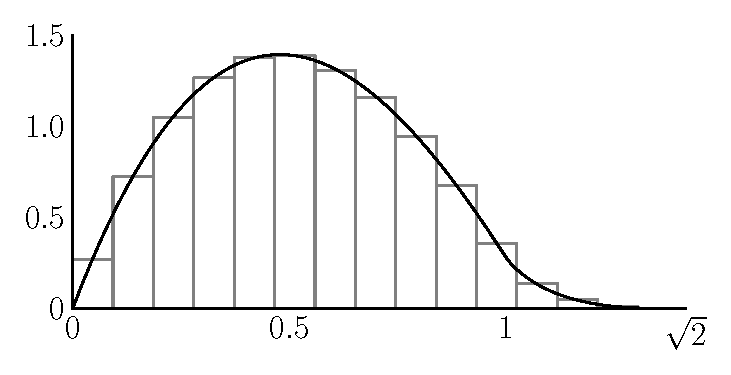
\includegraphics[width=0.7\textwidth, keepaspectratio]{%
    plots/01a179d9.pdf}%
  \label{fig:distance_distribution}
\end{figure}
%
\vspace{-0.8cm} Density functions \ref{eq:distance_square} and
\ref{eq:distance_unit_square} are of high importance. %?? Where when
Here we use \ref{eq:distance_unit_square} to compute the probability
that a random pair of vertices in the distance-dependent random graph
model is connected:

\begin{corollary}\label{th:distance_p} Let $v \neq w$ be vertices in an arbitrary
  realization of $G_{\Phi}(n,C)$. The probability $p$ for an edge
  from $v$ to $w$ is given by 
  \[
    p = \int_0^{\sqrt{2}} C(x) f(x) \, dx,
  \]
  where $f(x)$ is the probability density function~(\ref{eq:distance_unit_square}).
\end{corollary}

\textbf{Example} Let $C(x) = 1 - \frac{x}{\sqrt{2}}$. Then we compute
the probability to find an edge between a random vertex pair in
$G_{\Phi}(n,C)$ according to Theorem~\ref{th:distance_p} as
\[
  p = \int_{0}^{\sqrt{2}} f(x) \, dx - \frac{1}{\sqrt{2}}
  \int_0^{\sqrt{2}} x f_D(x) \, dx = 1 - \frac{1}{\sqrt{2}}\, \mathbf{E}[D].
\]
The expected distance between two random points on the unit square is
computed as $\mathbf{E}[D] \approx 0.521405$ (\autoref{mathematica:distances}),
a result confirmed by \textcite{Philip2007}. Thus we obtain the
probability for connection of $p \approx 0.631311$





% ######################################################################### %
% ------------------------------------------------------------------------- %
%                           Connectivity Matrix 
% ------------------------------------------------------------------------- %
% ######################################################################### %

% \section{Connectivity Matrix}



% An important concept in computation

% \begin{definition}[Connectivity matrix]
%   Let $G$ be a labeled directed graph with $n$ vertices. Then the
%   \textit{connectivity matrix} $A(G)$ of $G$, is a matrix such that
%   $A(G)_{ij} = 1$ if there exists an edge $e \in E(G)$ with $s(e)=i$
%   and $t(e)=j$ and $A(G)_{ij} = 0$ otherwise.
% \end{definition}

% Also known as \textit{adjacency matrix}. $\sum = degree$.


% From Graph clustering - Satu Elisa Schaeffer - 2007
% 
% [84] P. Erdos, A. Rényi, On random graphs I, in: Selected Papers
% of Alfréd Rényi, vol. 2, Akadémiai Kiadó, Budapest, Hungary,
% 1976, pp. 308–315. First publication in Publ. Math. Debrecen
% 1959.
% [85] P. Erdos, A. Rényi, On the evolution of random graphs,
% in: Selected Papers of Alfréd Rényi, vol. 2, Akadémiai Kiadó,
% Budapest, Hungary, 1976, pp. 482–525. First publication in
% MTA Mat. Kut. Int. Közl. 1960.





%%% Local Variables: 
%%% mode: latex
%%% TeX-master: "../dplths_document"
%%% End: 
